\documentclass{acmsiggraph}               % final

%% These two line bring in essential packages: ``mathptmx'' for Type 1
%% typefaces, and ``graphicx'' for inclusion of EPS figures.

\usepackage{graphicx}
\usepackage{url}
\usepackage{times}
\usepackage{ifpdf}


%% Paper title.

\title{Reflective Variance Shadow Maps}

\author{Gustaf Waldemarson\thanks{e-mail: ada09gwa@student.lu.se} \and Oguz Taskin\thanks{e-mail: ada09ota@student.lu.se}}
\affiliation{Faculty of Engineering (LTH), Lund University \\ Sweden}


%% Keywords that describe your work.
\keywords{Global Illumination, Reflective Shadow Maps, Variance Shadow Maps, Indirect Illumination, Color Bleeding}

%%%%%% START OF THE PAPER %%%%%%

\begin{document}

\ifpdf
  \DeclareGraphicsExtensions{.jpg,.pdf,.mps,.png}
\else
  \DeclareGraphicsExtensions{.eps}
\fi


\maketitle

\begin{abstract}
Lighting is a very important phenomenon in computer graphics, while basic direct lighting and shadowing algorithms provide an acceptable approximation to the light in the real world, they are unable to model more subtle lighting phenomena -- such as color bleeding and indirect illumination. Recently, a new use of the classic \emph{Shadow Map} has lead to a relatively simple algorithm, capable of introducing single bounce indirect illumination called \emph{Reflective Shadow Maps}. This paper focuses on the implementation of this algorithm, as well as that of another extension of the normal shadow map called \emph{Variance Shadow Maps} which can significantly smoothen the shadows in a wide variety of scenes.
\end{abstract}
\keywordlist

\section{Introduction}
Direct lighting have been used for a long time since they run very fast in real time applications. To create a greater feeling of realism, some kind of global illumination is required. The best approximation to global illumination is of course ray tracing algorithms such as \emph{Photon Mapping} or \emph{Path Tracing}. Neither of these approaches are interactive however, even with modern computer graphics hardware.

The Reflective Shadow Maps technique, described in Section~\ref{sec:rsm} is a very good starting point for global illumination since it can be run in real-time at interactive frame rates and is also used in more advanced illumination techniques such as \emph{Splatting Indirect Illumination} \cite{SII06} or \emph{Light Propagation Volumes} \cite{LPV09}.

Other techniques, such as \emph{radiosity}
%Need a source -- possibly ommitted%
are typically a lot faster than these approaches, but as a trade-off, these approaches usually need static lights in order to calculate the light propagation only once per scene. If the lights move, these time intensive calculations must be repeated.

Even with indirect illumination, interactive scenes will not look nearly as good if the shadows are \emph{blocky or pixelated}. These artefacts are often caused by the shadows cast by standard shadow maps. Techniques such as Percentage Closer Filtering \emph{(PCF)} can improve the look of the shadows, but only a ridiculously large filter can remove the blockyness at close inspection.

A very elegant solution to this is provided by the \emph{Variance Shadow Maps} technique. Which will be able to smoothen the shadows in a very satifying manner, while using only a small amount of extra memory.

Both of these algorithms were implemented in the \emph{RenderChimp} OpenGL (2) Renderer along with deferred rendering code from laboratory 2 in the course \emph{EDAN35} --- High Performance Computer Graphics.

\section{Reflective Shadow Maps -- RSM}
\label{sec:rsm}
The Reflective Shadow Map introduced by \cite{RSM2005} is essentially an extension of the regular shadow map but this technique uses the contents of it in a different way in order to introduce indirect illumination. Instead of just containing the depth from the light source, this shadow map contains the following things in additional buffers:

\begin{description}
	\item[Normals] The world-space normals on points seen by the light source.
	\item[Flux] The total amount of reflective radiant flux from the points seen by the light source. An example of how this looks can be seen in Figure~\ref{fig:flux}.
\end{description}

\begin{figure}[tb]
    \centering
    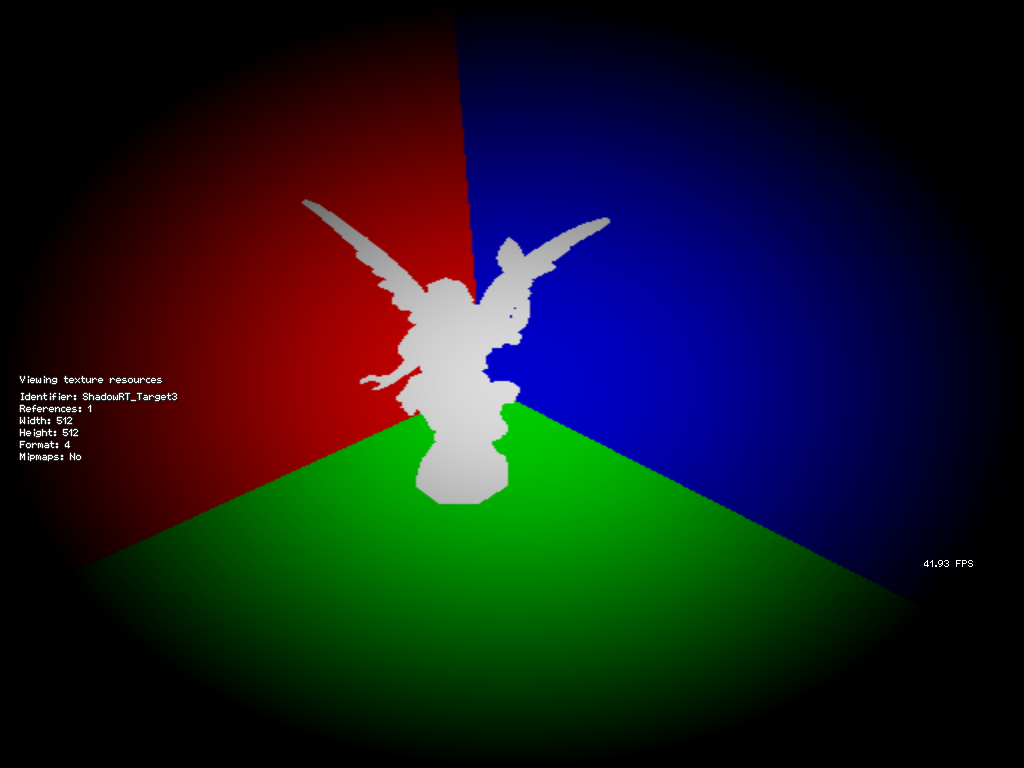
\includegraphics[width=0.7\columnwidth]{./images/flux.png}
    \caption{Image showing what our flux-buffer looks like. Note that the values in this example are deliberately chosen to emphasize the effect.}
    \label{fig:flux}
\end{figure}

In a subsequent render pass, the indirect illumination is accumulated in a texture by querying for the depth, normal and flux at a large amount of positions sampled with the scheme described in Section~\ref{sec:optrsm}. This accumulated lighting is then added to the ambient lighting in the scene, giving an impression of indirect illumination.

\subsection{Optimization - Sampling Scheme}
\label{sec:optrsm}
For each pixel in screen space, the indirect lighting is calculated by querying the \emph{RSM} a large number of times\footnote{Our approach uses $400$ samples.}. Since the relevant sources of indirect illumination could be anywhere in the scene, a random sampling scheme was used to increase the probability of sampling from such a region. See figure~\ref{fig:samp} for an illustration of the scheme.

\begin{figure}[tb]
    \centering
    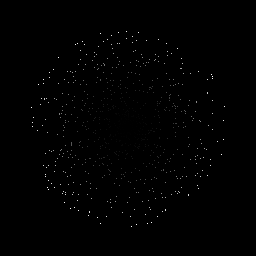
\includegraphics[width=0.7\columnwidth]{./images/sampling.png}
    \caption{Image of the sampling pattern. The brightness of the point represent the weight of the sample.}
    \label{fig:samp}
\end{figure}

This scheme could have been exported directly as an image and read as a texture by a shader but in order to reduce the bandwidth, a simpler, $1$ dimensional RGBA8 texture was exported instead. In this texture, the Red and Green channels contain the $x$ and $y$ coordinates respectively and the weight was stored in the Blue channels. A more efficient scheme could potentially generate these values procedurally instead if the hardware had access to efficient \emph{noise} functions.\footnote{This kind of sampling schemes may however have a large impact on the bandwidth when reading from the \emph{RSM}, since they completely disregard temporal and spatial locality utilized by caching algorithms. It could be alleviated however, by storing the sample points in an order better utilized by the cache.}

\section{Variance Shadow Maps -- VSM}
\label{sec:vsm}
Variance Shadow Maps is another extension to the basic shadow map, solving some of the problems encountered by the standard one, such as the biasing, while giving features such as very smooth edges. To generate this enhanced shadow map, we attach the camera on the light source as usual, but instead of generating just the depth, we also generate and save the squared depth in the buffer. These will then be treated as \emph{statistical moments}.

Generally, shadow maps cannot be filtered using the available hardware filtering algorithms, both \emph{Nvidia} and \emph{AMD} however, do provide filtering of shadow maps on certain GPUs, but these often cause aliasing or other artefacts. This is caused by the fact that depth values cannot be correctly interpolated, as described by \cite{VSM2006} but statistical moments \emph{can} be accurately interpolated with hardware filtering since they describe a distribution instead.

To use these moments, the one-tailed Chebyshev Inequality is computed to describe the \emph{probability} of the point being directly lit by the light source. It is computed as follows:

\begin{equation}
	P(x \geq t) \leq p_{max}(t) = \frac{\sigma^2}{\sigma^2 + (t - \mu)^2}
\end{equation}

Where $\sigma^2$ is the depth squared, or the second moment. $\mu$ is the regular shadow map depth, or the first moment, and $t$ is the depth for the current point. If this probability is low, the point is assumed to be in shadow. Otherwise, the light is attenuated by this probability, giving us a smooth edge, or a fake penumbra.

If the texture is filtered with a Gaussian blurring algorithm such as \cite{GGGauss07} or with a simple box-filter, the shadow gradient could be improved even further.

\subsection{Summed Area Variance Shadow Maps}
Hardware filtering is not always available, but smoothing can still be done with the help of Summed Area Tables \emph{(SAT)} as seen in \cite{GGVSM07} which are generated as in \cite{FSAT05}. The generation of this table is however a great concern, since SATs require a very high amount of precision. Since \emph{RenderChimp} is limited to \emph{RGBA8} textures at this time, this feature was not implemented.

\section{Results}
A few of the images generated with our algorithms can be seen in figures~\ref{fig:noind}, \ref{fig:daind} and \ref{fig:oind}. Note that the color bleeding is greatly emphasized in these pictures in order to clearly show the effects of the indirect illumination. Several other images can be seen in Figures~\ref{fig:ang1}, \ref{fig:ang2} and \ref{fig:ang3} at the bottom of this paper.

\begin{figure}[tb]
    \centering
    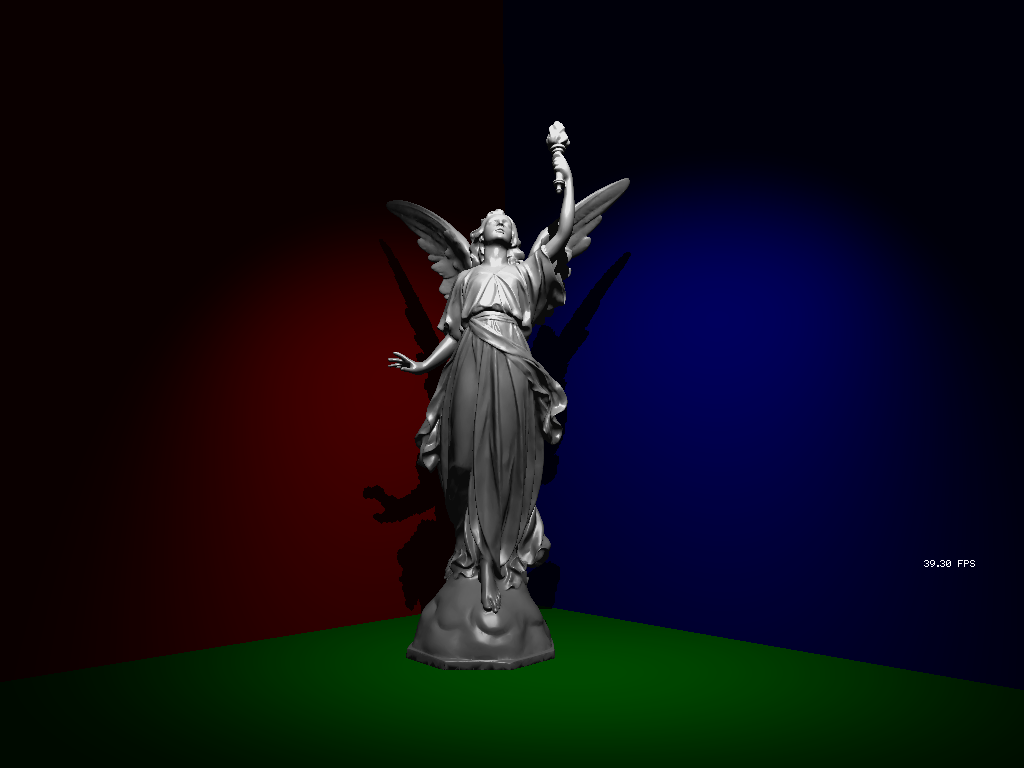
\includegraphics[width=0.7\columnwidth]{./images/p1-A.png}
    \caption{Stanford Lucy without any indirect illumination.}
    \label{fig:noind}
\end{figure}

\begin{figure}[tb]
    \centering
    
\includegraphics[width=0.7\columnwidth]{./images/p1-B.png}
    \caption{Stanford Lucy with direct and indirect illumination. Note that the color bleeding is greatly enhanced in this image in order to visualize the effects.}
    \label{fig:daind}
\end{figure}

\begin{figure}[tb]
    \centering
    
\includegraphics[width=0.7\columnwidth]{./images/p1-gi-exp.png}
    \caption{Stanford Lucy with \emph{only} indirect illumination. Note that the illumination is greatly enhanced to visualize the effects.}
    \label{fig:oind}
\end{figure}


\section{Discussion}
\subsection{Reflective Shadow Maps}
The most important part of Global Illumination is obviously the first bounce of the light by the diffuse reflector. This is exactly what the Reflective Shadow Maps approximates, giving us the most important aspect of it in real time. It is however limited to a single bounce and certain aspects, such as \emph{indirect shadows}, are not captured at all by just the RSM. It is however, largely independent of the geometry of the scene, and is thus very applicable in applications were light sources can move or a large amount of objects can move around. Also, the effectiveness of the color bleeding from the flux is limited when the scene uses textures with varying colors.


\subsection{Variance Shadow Maps}
Variance Shadow Maps is a very simple extension of the original shadow map and only requires a small amount of extra bandwidth to give the shadows a very smooth look. Coupled with a blurring function, even very small shadow maps, such as a map of size $128$ by $128$ will still have a very smooth shadow when properly blurred. The shadow from such a small shadow map will however lose a lot of the details, but the improved performance along with the smooth shadows might be more appropriate for some applications.

\section{Conclusion}
Reflective Shadow Maps is an interesting algorithm, it is the logical starting point for any kind of global illumination for applications with dynamic lights, such as video games. In these cases, the indirect light is often not very noticeable, but the absence of it is. Without it, many scenes will look unrealistically dark.

Even with the added lighting however, shadows that are more realistic than the ones provided by standard shadow maps are required to further enhance the result of the indirect illumination. Variance Shadow Maps can provide such an improvement with only a small spatial and computational complexity added. In fact, it is so simple to add the basic VSM algorithm on top of the standard Shadow Maps, that there is little reason to implement \emph{just} shadow maps when adding shadowing algorithms to any graphics application.

\newpage

\begin{figure}[p]
    \centering
    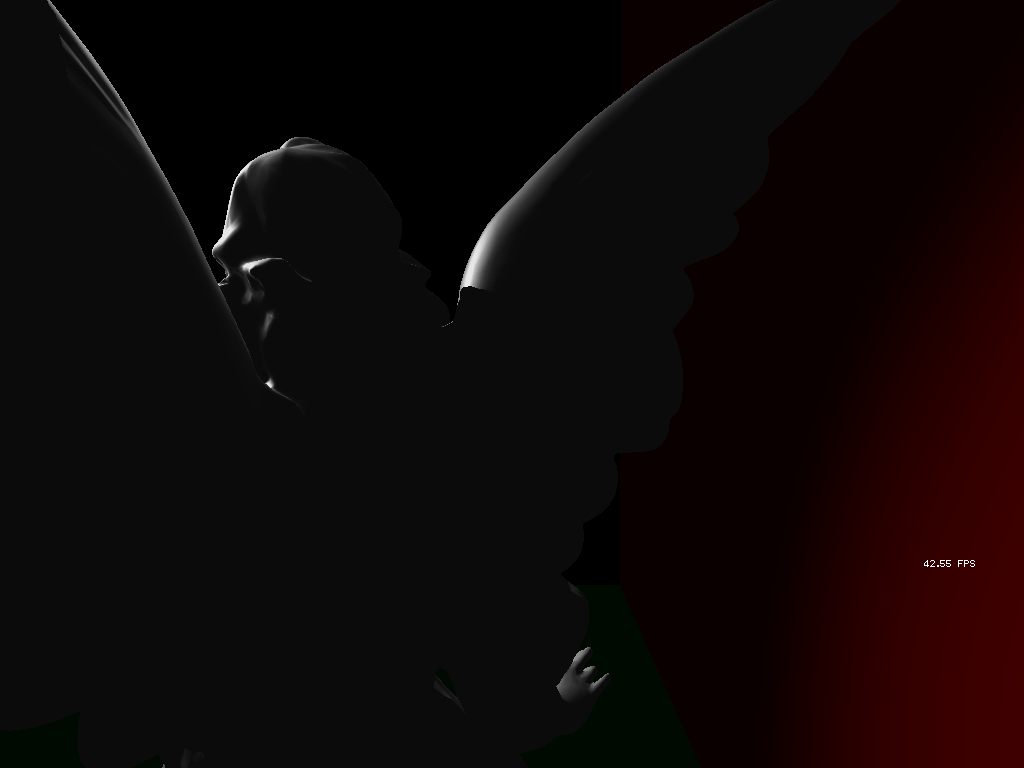
\includegraphics[width=1.0\columnwidth]{./images/p2-A.png}
    \caption{Stanford Lucy without any indirect illumination.}
    \label{fig:ang1}
\end{figure}

\begin{figure}[p]
    \centering
    
\includegraphics[width=1.0\columnwidth]{./images/p2-B.png}
    \caption{Stanford Lucy with direct and indirect illumination. The camera is positioned behind Lucy to clearly show the color bleeding from the walls onto her.}
    \label{fig:ang2}
\end{figure}

\begin{figure}[p]
    \centering
    
\includegraphics[width=1.0\columnwidth]{./images/p2-gi-exp.png}
    \caption{Stanford Lucy with \emph{only} indirect illumination.}
    \label{fig:ang3}
\end{figure}



%List of all citations to avoid warnings from TeX. %
\cite{VSM2006,RSM2005,GGGauss07,GGVSM07,FSAT05}

\bibliographystyle{acmsiggraph}
%\nocite{*}
\bibliography{project}
\end{document}



